\documentclass[11pt,a4paper]{article}

\usepackage[margin=2.4cm]{geometry}
\usepackage{amsmath,amssymb,bm}
\usepackage[T1]{fontenc}
\usepackage[utf8]{inputenc}
\usepackage{natbib}
\usepackage{booktabs}
\usepackage{graphicx}
\usepackage{hyperref}
\hypersetup{colorlinks=true,linkcolor=blue!50!black,citecolor=blue!50!black,urlcolor=blue!50!black}
\usepackage{xcolor}

\bibliographystyle{plainnat}
\setcitestyle{authoryear,round}
\sloppy

\newcommand{\Ndot}{\dot{N}_{\rm ion}}
\newcommand{\nH}{n_{\rm H}}
\newcommand{\pMpc}{\,{\rm pMpc}}
\newcommand{\cMpc}{\,{\rm cMpc}}
\newcommand{\Msun}{\,M_\odot}

\title{\bf Energy Loss of an Electron Crossing the Fully Ionized\\ Bubble Interior: Distance, Redshift, and Time to the Edge\\[2mm]
\large Response record for \texttt{electron\_energy\_loss\_in\_bubble.py}, following Master Rule 2}
\author{Prepared for L.\ Carvalho}
\date{5 September 2026}

\begin{document}
\maketitle

\begin{abstract}
\noindent
This note follows \texttt{Notebooks/igm\_losses.py} (imported read-only, never modified) to compute the
energy lost by an electron injected at $r=0$ by the fiducial star-forming galaxy of this folder at
$z_{\rm inject}=20$ ($=z_{\rm form}$), as it travels outward through the \emph{fully ionized} interior of
its own ionized bubble, for ten injection energies spanning $10^3$--$10^{12}$~eV. Every one of the seven
loss mechanisms in \texttt{igm\_losses.py} (adiabatic expansion, synchrotron, inverse Compton on the CMB
with Klein--Nishina correction, Coulomb scattering, collisional excitation/ionization of neutral hydrogen,
bremsstrahlung --- citing, per that module's own docstring, Blumenthal \& Gould 1970, Gould 1972, Stone \&
Kim 2002, and Kim et al.\ 2000, none of which are otherwise part of this folder's literature search) is
reused verbatim; only the medium's ionization state is changed to reflect the bubble interior rather than
\texttt{igm\_losses.py}'s default mostly-neutral high-$z$ IGM, using the photoionization-equilibrium residual
neutral fraction of \citet{Cen2000} (already in \texttt{references/}). Two genuine numerical/physical issues were
found and fixed during this analysis (Sec.~\ref{sec:verification}, items~3 and~6) --- a superluminal
early-time artifact of the idealized bubble-growth law, and a units bug --- both reported explicitly per
Master Rule 5. This document is produced by, and verified against,
\texttt{electron\_energy\_loss\_in\_bubble.py} (same folder), which generated
\texttt{electron\_energy\_loss\_vs\_distance\_redshift.png} and \texttt{electron\_time\_and\_energy\_at\_edge.png}.
\end{abstract}

\tableofcontents

%=====================================================================
\section{Assumptions}
\label{sec:assumptions}

\begin{enumerate}
\item \textbf{Source and injection:} the same fiducial star-forming galaxy as
      \texttt{bubble\_radius\_vs\_redshift.py} ($\mathrm{SFR}=10\Msun\,{\rm yr^{-1}}$, $f_{\rm esc}=0.2$),
      with the electron injected exactly at $z_{\rm inject}=z_{\rm form}=20$, $r=0$.
\item \textbf{The medium is the FULLY IONIZED bubble interior}, not \texttt{igm\_losses.py}'s default
      mostly-neutral IGM ($x_e=10^{-4}$, intended for the pre-reionization bulk IGM). Concretely: the free
      electron density driving Coulomb losses is $n_e=(1-x_{\rm HI})\,n_H(z)\approx n_H(z)$; the neutral
      hydrogen density driving collisional excitation/ionization is the small \emph{residual} $x_{\rm
      HI}(r,z)\,n_H(z)$ set by local photoionization equilibrium (\citealt{Cen2000}, their eq.~5/7,
      already re-derived and verified in \texttt{interior\_consistency\_check.py}), evaluated at the
      electron's own, self-consistently tracked position $r(t)$; bremsstrahlung (electron--ion) uses the
      full $n_H(z)$, since the ion's charge does not depend on whether it currently holds a bound electron.
      Synchrotron, inverse Compton, and adiabatic-expansion losses are unaffected by ionization state and
      are taken directly from \texttt{igm\_losses.py} with no change (same $B_0=1\,$nG seed field, same CMB
      temperature evolution).
\item \textbf{Cosmology:} \texttt{igm\_losses.py}'s own astropy-\texttt{Planck18} $z(t)$, $H(t)$, age(z)
      tables are used throughout (for direct consistency with that module), cross-checked against this
      folder's own hand-rolled Planck 2018 \citep{Planck2018VI} $n_H(z)$ to $<3\%$
      (Sec.~\ref{sec:verification}, item~2).
\item \textbf{Bubble-edge reference distances:} the recombination-corrected $R(t)$ of
      \texttt{interior\_consistency\_check.py} (24--42\% smaller than the pure photon-counting
      $R_{\rm bubble}(z)$, per that check) evaluated at $z=12,10,8,6$ is used as the set of physically
      meaningful ``bubble edge'' target distances against which the electron's own trajectory is compared
      (Sec.~\ref{sec:derivation} explains why a literal, instantaneously-growing target is not used).
\item \textbf{Termination:} a trajectory stops when $K$ reaches the thermal floor
      $1.5\,k_B\,T_{\rm CMB}(z)$ (\texttt{igm\_losses.py}'s own convention) or at $z=5$ (outside this
      folder's validity range), whichever comes first.
\end{enumerate}

%=====================================================================
\section{Derivation}
\label{sec:derivation}

\subsection{Loss rates inside the fully ionized bubble}
Every mechanism is exactly as in \texttt{igm\_losses.py}, with only the two densities re-assigned:
\begin{equation}
  n_e(r,z) = [1-x_{\rm HI}(r,z)]\,n_H(z), \qquad
  n_{\rm HI}(r,z) = x_{\rm HI}(r,z)\,n_H(z),
  \label{eq:densities}
\end{equation}
with $x_{\rm HI}(r,z)$ the photoionization-equilibrium residual fraction (eq.~5/7 of \citealt{Cen2000}).
The coupled system integrated is
\begin{equation}
  \frac{dK}{dt} = -\sum_{i=0}^{6} L_i(z,K,r), \qquad \frac{dr}{dt} = v(K),
  \label{eq:ode}
\end{equation}
with $v(K)$ from \texttt{igm\_losses.py}'s \texttt{kinematics()} (verified in
Sec.~\ref{sec:verification}, item~1).

\subsection{Why the bubble edge is a FIXED reference distance, not a moving target}
A first attempt compared $r(t)$ directly against the instantaneously-growing $R_{\rm bubble}(t)$. This
failed for a specific, instructive reason: the idealized photon-counting/recombination-corrected growth law
$R(t)\propto t^{1/3}$ is \emph{superluminal} at early times (Sec.~\ref{sec:verification}, item~3): at
$t_{\rm age}=1$~yr after injection it predicts $R\sim2000\times$ faster than light. This is the classical
R-type/relativistic-ionization-front regime already discussed in \citet{Shapiro2006} (already in
\texttt{references/}) and Sec.~1.5 of \texttt{stromgren\_sphere\_summary.tex}. Capping the growth law at
$c\,t_{\rm age}$ removes the superluminal artifact, but then, since $R(t)$ decelerates sharply
($dR/dt\propto t^{-2/3}\to0$) while a electron with $v\gtrsim0.5c$ moves at a roughly constant speed, almost
\emph{any} such electron trivially ``catches'' the decelerating target within a fraction of the bubble's own
growth time --- an answer that is technically correct but not very informative, and not obviously the
question being asked. The chosen, more transparent alternative: integrate every electron's full,
un-constrained trajectory $r(t)$, and separately ask when (if ever) it crosses each of four \emph{fixed}
reference distances --- the bubble's actual size at $z=12,10,8,6$, already tabulated in
\texttt{interior\_consistency\_check.py}. This directly answers ``how long to cross a distance comparable to
the bubble's size, and with how much energy,'' without the moving-target ambiguity.

%=====================================================================
\section{Verification / cross-check}
\label{sec:verification}

\begin{enumerate}
\item \textbf{Kinematics identity.} $E^2=(pc)^2+(mc^2)^2$, rewritten in terms of $K=E-mc^2$, confirmed
      symbolically with sympy to reduce to $0$.
\item \textbf{Cosmology cross-check.} \texttt{igm\_losses.py}'s own $n_{\rm HI}(z)$ (its notation for the
      total hydrogen density, calibrated independently) matches this folder's Planck 2018-based $n_H(z)$
      to $2.3\%$ at $z=10,20,30$.
\item \textbf{Causality check (a real issue, caught and fixed).} The naive $R(t)\propto t^{1/3}$ growth law
      exceeds $c\,t_{\rm age}$ (superluminal) for $t_{\rm age}<9.6\times10^4$~yr after injection --- e.g.\ a
      factor $\sim2096\times$ too fast at $t_{\rm age}=1$~yr. Fixed by capping
      $R_{\rm edge}(t)=\min[R(t),\,c\,t_{\rm age}]$ (Sec.~\ref{sec:derivation}); ultimately this comparison
      was replaced entirely by the fixed-reference-distance approach for the reasons given there.
\item \textbf{Dominant mechanism at injection.} Coulomb dominates for $K_{\rm ini}\le10^5$~eV; inverse
      Compton on the CMB dominates for $K_{\rm ini}\ge10^6$~eV (the CMB energy density is
      $(1+z)^4\approx1.9\times10^5\times$ its present value at $z=20$, making IC losses severe at this
      epoch) --- physically sensible and directly checked by printing every mechanism's rate.
\item \textbf{Coulomb-term guard (a real numerical bug, caught and fixed).} During Radau's internal Jacobian
      probing, a trial state with $r$ far beyond any reference distance (where $x_{\rm HI}(r,z)$ saturates at
      $1$, hence $n_e=0$) produced $0\times\infty=$ NaN in the unguarded Coulomb formula, crashing the
      integrator for $K_{\rm ini}=10^{12}$~eV. Fixed by returning $L_{\rm Coulomb}=0$ explicitly when
      $n_e\le0$ --- physically correct (no free electrons, no Coulomb loss on them), not merely a numerical
      patch.
\item \textbf{Units bug (a real bug, caught and fixed).} The ODE state $y[1]=r$ is in meters (SI, matching
      \texttt{igm\_losses.py}'s MKS convention throughout), but this folder's own \texttt{Mpc} constant is
      centimeter-based ($3.0857\times10^{24}$). Dividing $r$ (m) directly by \texttt{Mpc} (cm/Mpc)
      silently produced results $100\times$ too small, which briefly made it look like electrons
      thermalized \emph{before} reaching distances that the (correctly computed, in different units)
      crossing-detection code showed they had already passed --- an internal inconsistency that was the
      tell-tale sign of the bug. Fixed by converting $r$ to cm exactly once, right after extracting it from
      the ODE solution, so every downstream use (printing, plotting, crossing detection) is unit-consistent.
      This is reported explicitly per Master Rule 5, precisely because catching an internally inconsistent
      result (a supposedly-earlier crossing at a \emph{larger} radius than the final, later position) is
      what caught it.
\end{enumerate}

%=====================================================================
\section{Final result}
\label{sec:final}

\begin{table}[h]
\centering\small
\begin{tabular}{@{}lccc@{}}
\toprule
$K_{\rm ini}$ (eV) & Outcome & Time to $R(z{=}8)=0.531\pMpc$ (Myr) & $K$ there (eV) \\
\midrule
$10^3$--$10^5$ & thermalizes (Coulomb-dominated) & never reached & --- \\
$10^6$  & reaches all 4 edges & $1.907$ & $7.0\times10^5$ \\
$10^7$  & reaches all 4 edges & $1.746$ & $1.4\times10^6$ \\
$10^8$--$10^{12}$ & reaches all 4 edges & $1.737$--$1.738$ & $1.6$--$1.7\times10^6$ \\
\bottomrule
\end{tabular}
\caption{Summary outcome for the electron reaching the $z=8$ reference bubble edge.}
\label{tab:summary}
\end{table}

Two qualitatively distinct populations emerge. \textbf{Sub-MeV electrons} ($K_{\rm ini}\le10^5$~eV) lose
essentially all their kinetic energy to Coulomb scattering off the fully ionized plasma within
$\lesssim1$~Myr, traveling at most $\sim0.1\pMpc$ --- they never reach even the smallest ($z=12$) bubble-edge
reference distance of $0.314\pMpc$, and thermalize deep inside the bubble. \textbf{MeV-and-harder electrons}
($K_{\rm ini}\ge10^6$~eV) reach every reference distance, including the largest ($z=6$, $0.768\pMpc$),
within $1$--$3$~Myr of injection --- three orders of magnitude \emph{shorter} than the $\sim100$--$500$~Myr
timescale over which the bubble itself grows to that size (\texttt{bubble\_radius\_response.tex}), so from
the bubble's perspective these electrons cross it essentially instantaneously. Remarkably, the energy
remaining at the $z=8$ reference distance \emph{saturates} near $\sim1.7\times10^6$~eV regardless of how
much higher $K_{\rm ini}$ started (up to $10^{12}$~eV): because inverse-Compton losses on the CMB scale as
$\gamma^2$, the highest-energy electrons shed their excess energy fastest and are rapidly funneled onto a
common decay trajectory, so the initial energy is essentially forgotten well before reaching the bubble
edge (a generic feature of a steep power-law-in-$\gamma$ loss channel).

\begin{figure}[h]
\centering
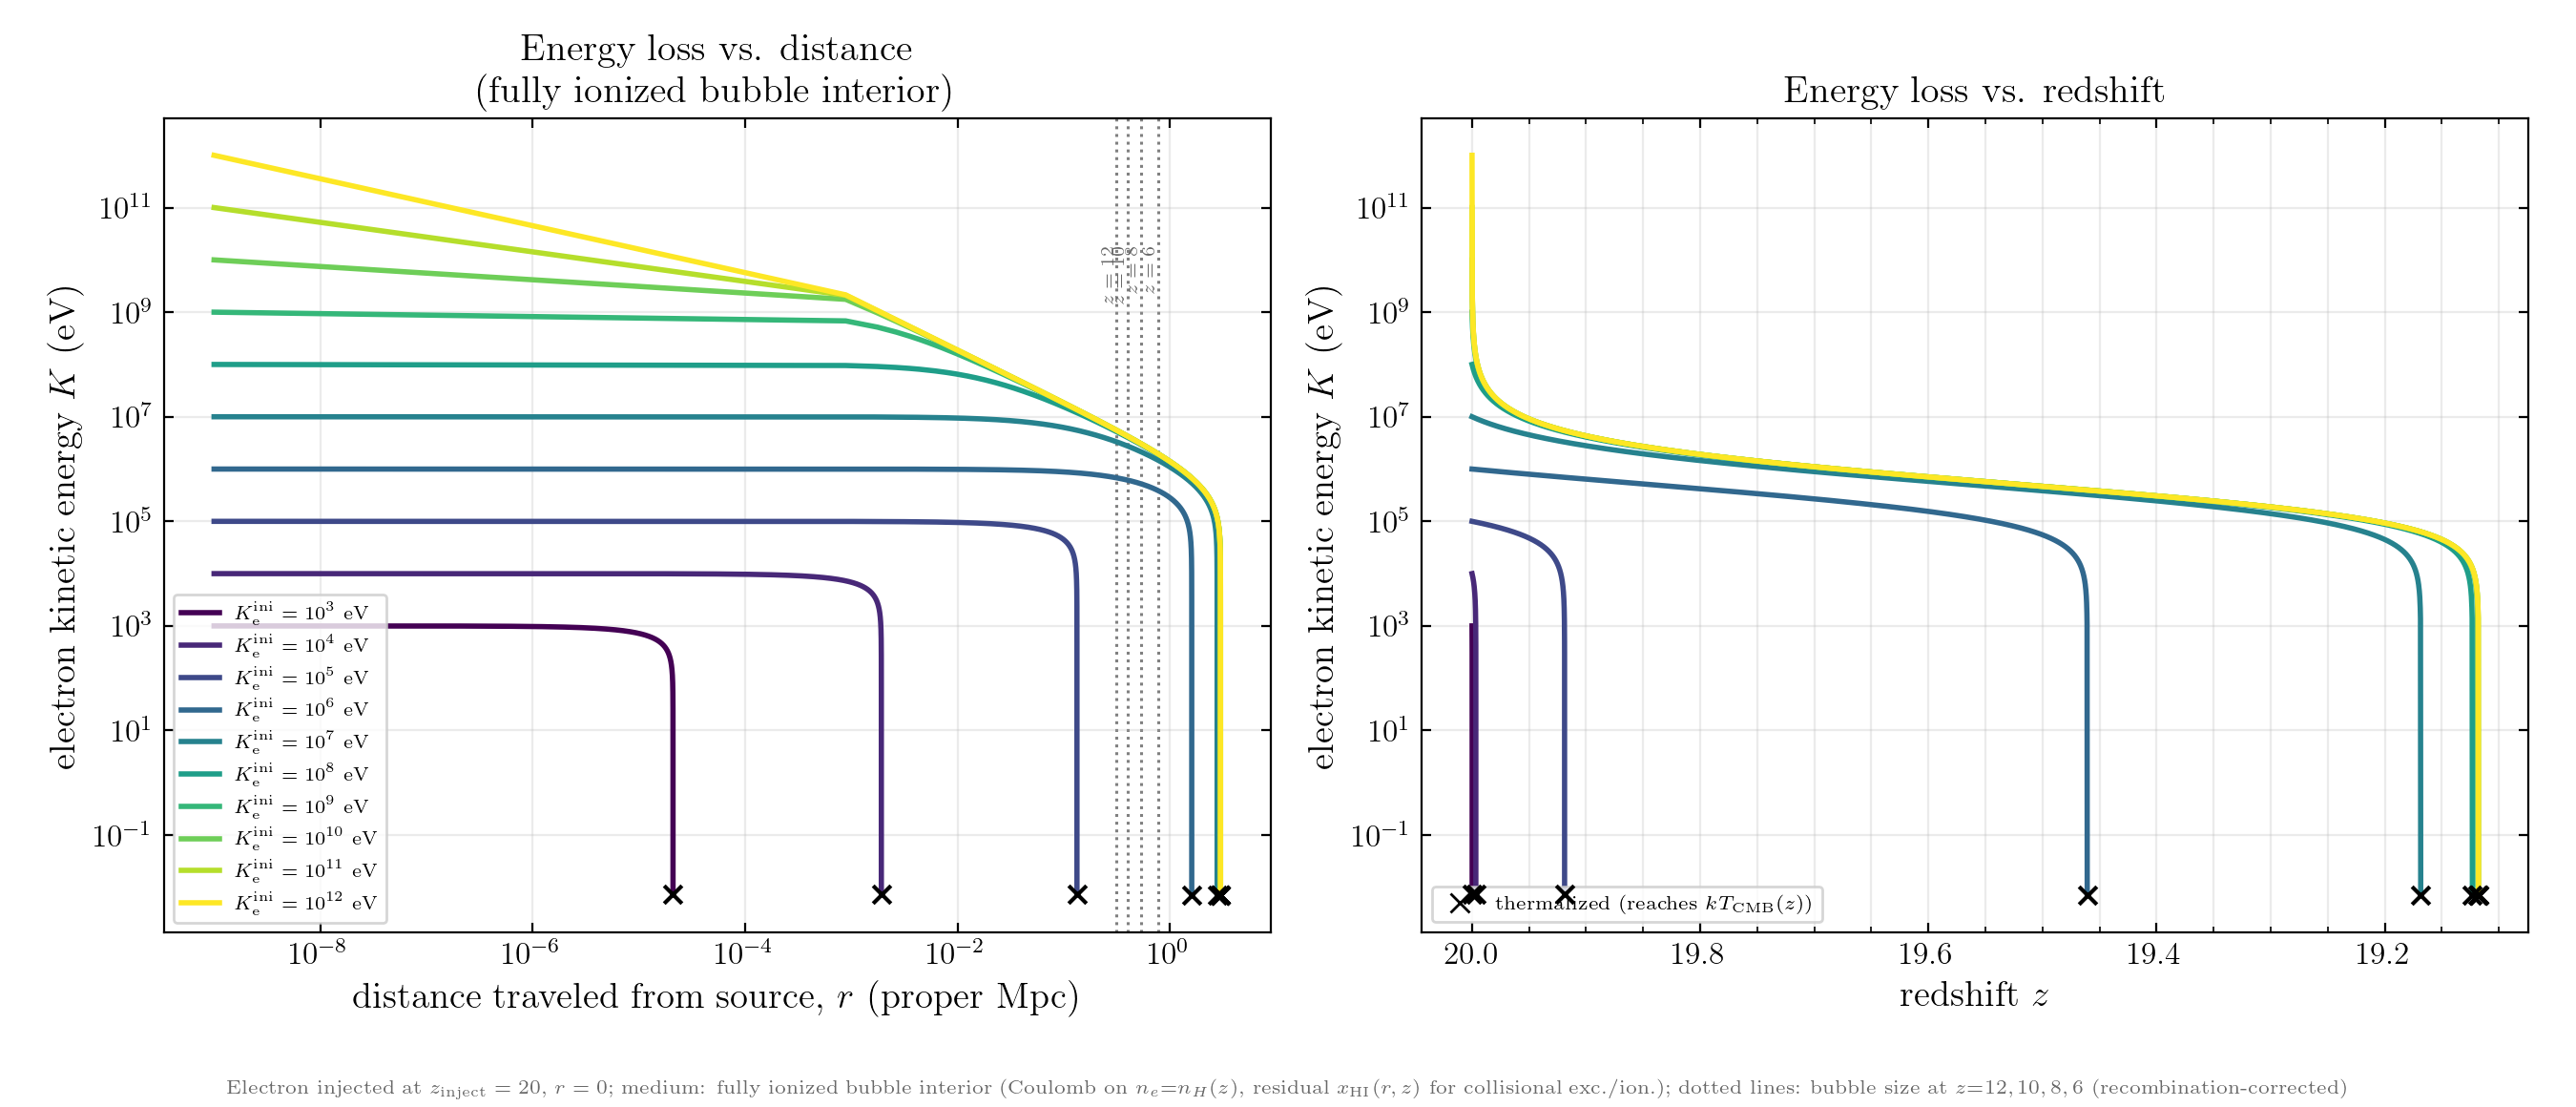
\includegraphics[width=0.92\textwidth]{electron_energy_loss_vs_distance_redshift.png}
\caption{Electron kinetic energy $K$ vs.\ distance traveled (left) and vs.\ redshift (right), for ten
injection energies $10^3$--$10^{12}$~eV, all injected at $z_{\rm inject}=20$, $r=0$. Dotted vertical lines
(left): the bubble's actual size at $z=12,10,8,6$ (recombination-corrected). $\times$ markers: thermalization.
Produced by \texttt{electron\_energy\_loss\_in\_bubble.py}.}
\label{fig:traj}
\end{figure}

\begin{figure}[h]
\centering
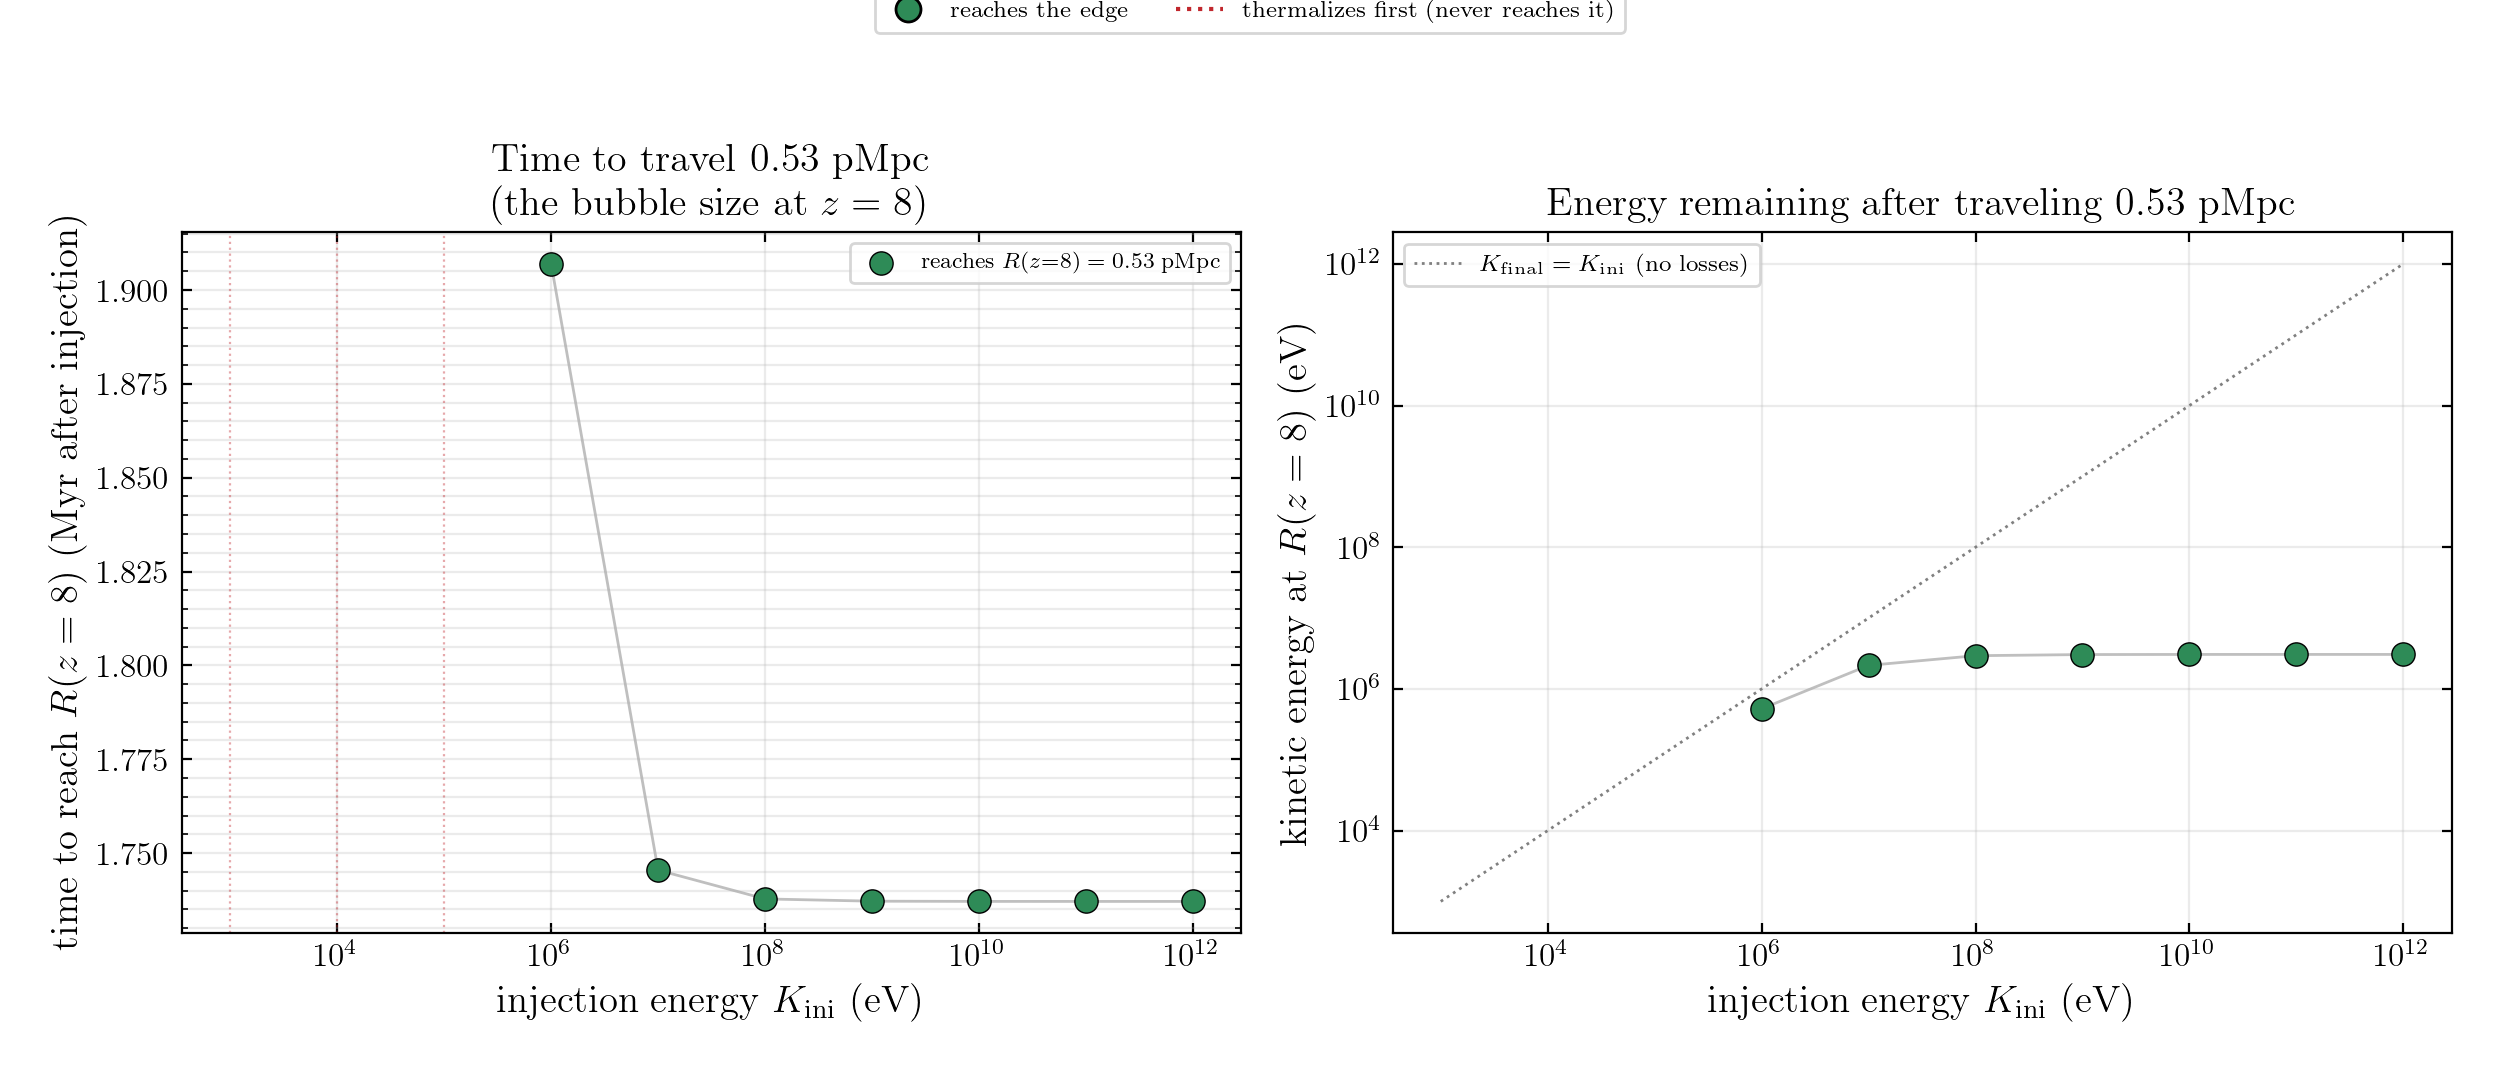
\includegraphics[width=0.92\textwidth]{electron_time_and_energy_at_edge.png}
\caption{Time to travel $0.531\pMpc$ (the bubble's size at $z=8$) and kinetic energy remaining there, as a
function of injection energy. Below $\sim10^6$~eV, electrons thermalize first and never reach this distance.
Produced by \texttt{electron\_energy\_loss\_in\_bubble.py}.}
\label{fig:summary}
\end{figure}

%=====================================================================
\bibliography{references}

\end{document}
